\documentclass{beamer}

\mode<presentation>
{
  \usetheme{CambridgeUS}
  \setbeamercovered{transparent}
}

\usepackage[english]{babel}
\usepackage[latin1]{inputenc}
\usepackage{times}
\usepackage[T1]{fontenc} 
% Or whatever. Note that the encoding and the font should match. If T1
% does not look nice, try deleting the line with the fontenc.
\usepackage{amsmath}

\newcommand{\linespace}{\vskip 0.25cm}

\definecolor{MyForestGreen}{rgb}{0,0.7,0}
\newcommand{\tableemph}[1]{{#1}}
\newcommand{\tablewin}[1]{\tableemph{#1}}
\newcommand{\tablemid}[1]{\tableemph{#1}}
\newcommand{\tablelose}[1]{\tableemph{#1}}

\definecolor{MyLightGray}{rgb}{0.6,0.6,0.6}
\newcommand{\tabletie}[1]{\color{MyLightGray} {#1}}

% The text in square brackets is the short version of your title and will be used in the
% header/footer depending on your theme.
\title[Mobile Security]{Gait Recognition in Mobile Security}

% Sub-titles are optional - uncomment and edit the next line if you want one.
% \subtitle{Why does sub-tree crossover work?} 

% The text in square brackets is the short version of your name(s) and will be used in the
% header/footer depending on your theme.
\author[Ottomoeller]{Chase R. Ottomoeller}

% The text in square brackets is the short version of your institution and will be used in the
% header/footer depending on your theme.
\institute[U of Minn, Morris]
{
  Division of Science and Mathematics \\
  University of Minnesota, Morris \\
  Morris, Minnesota, USA
}

% The text in square brackets is the short version of the date if you need that.
\date[December '14, SS, Morris] % (optional)
{December 6, 2014 \\ Senior Seminar, Morris}

% Delete this, if you do not want the table of contents to pop up at
% the beginning of each subsection:
\AtBeginSection[]
{
  \begin{frame}<beamer>
    \frametitle{Outline}
    \tableofcontents[currentsection, hideothersubsections]
  \end{frame}
}

\begin{document}

\begin{frame}
  \titlepage
\end{frame}

% For a 20-25 minute senior seminar talk you probably want something like:
% - Two or three major sections (other than the summary).
% - At *most* three subsections per section.
% - Talk about 30s to 2min per frame. So there should probably be between
%   15 and 30 frames, all told.

\section*{Overview}

\subsection*{The Big Picture}

\begin{frame}
  \frametitle{The Big Picture}
  
  \begin{columns}
  \begin{column}{0.6\textwidth}
  What is Mobile Security?
     \begin{itemize}
     \item Information Storage
  	  \item Device Access 
  	  \linebreak
     \end{itemize}
     
  How is mobile security evolving?
     \begin{itemize}
     \item No More Passwords
	  \item Something You Are
%	\item What is Gait Recognition?
%	\item How is Gait Recognition useful?
     \end{itemize}
  \end{column}
  \begin{column}{0.4\textwidth}
   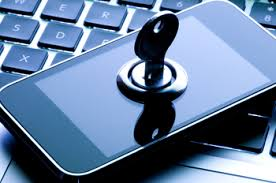
\includegraphics[width=0.95\textwidth]{Illustrations/mobileSecurity.jpg}
       \\
    \only{\tiny{ http://mobilebuzz.guru/wp-content/uploads/2014/06/Mobile-Security.png} }
  \end{column}
  \end{columns}
\end{frame}

\subsection*{Outline}

\begin{frame}
  \frametitle{Outline}
  \tableofcontents[hideallsubsections]
\end{frame}





\section[Mobile Security]{Background}

\subsection{Biometrics}
\begin{frame}
  \frametitle{Biometrics}

  \begin{columns}
  \begin{column}{0.4\textwidth}
  \begin{itemize}
    \item Biometrics 
  	\linebreak
  	\item Gait Recognition
  	\linebreak
	\item Why Gait is Better
	\linebreak
	\item Unobtrusive Access
  \end{itemize}
  \end{column}
  \begin{column}{0.8\textwidth}
   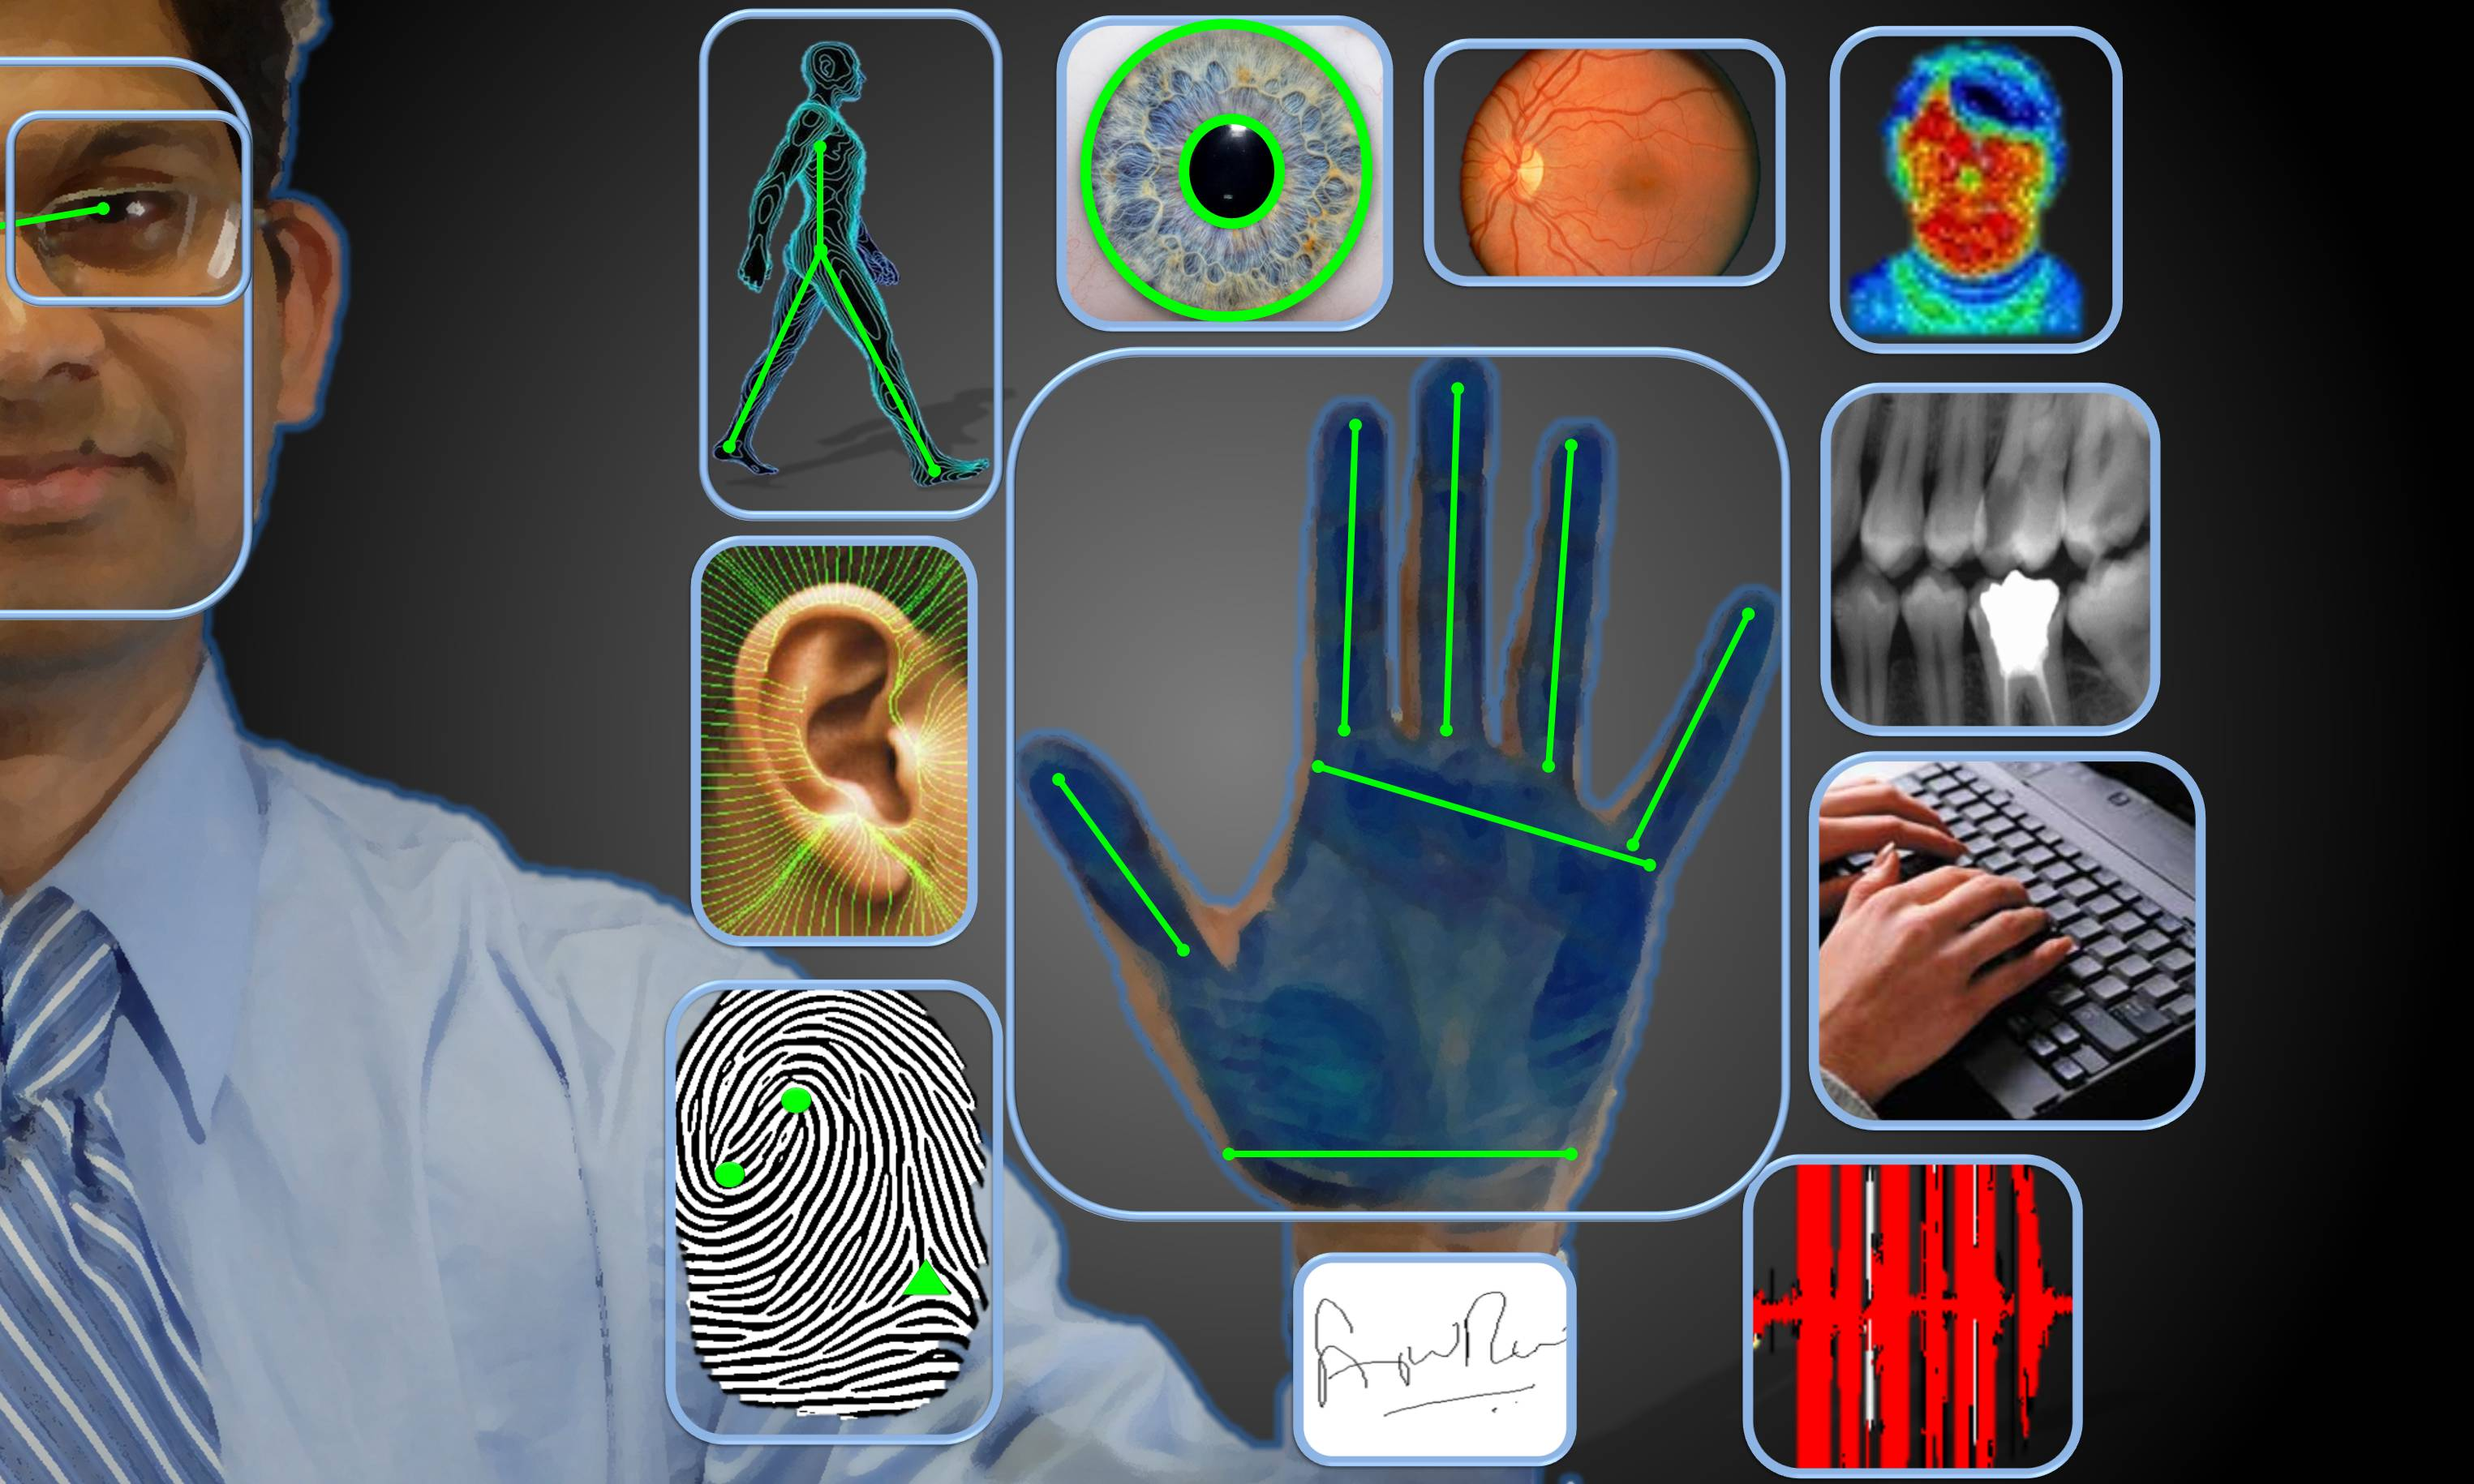
\includegraphics[width=0.8\textwidth]{Illustrations/allbiometrics.jpg}
       \only{\tiny{ http://www.smc2012.org/images/jain3-1.jpg} }
  \end{column}
  \end{columns}
\end{frame}

\subsection{Two Methods}

\subsection{}
\begin{frame}
  \frametitle{Two Methods}
  \begin{columns}
  \begin{column}{0.4\textwidth}
  \begin{itemize}
    \item Fixed Method
  	\linebreak
  	\item Unfixed Method
  \end{itemize}
  \end{column}
  \begin{column}{0.8\textwidth}
   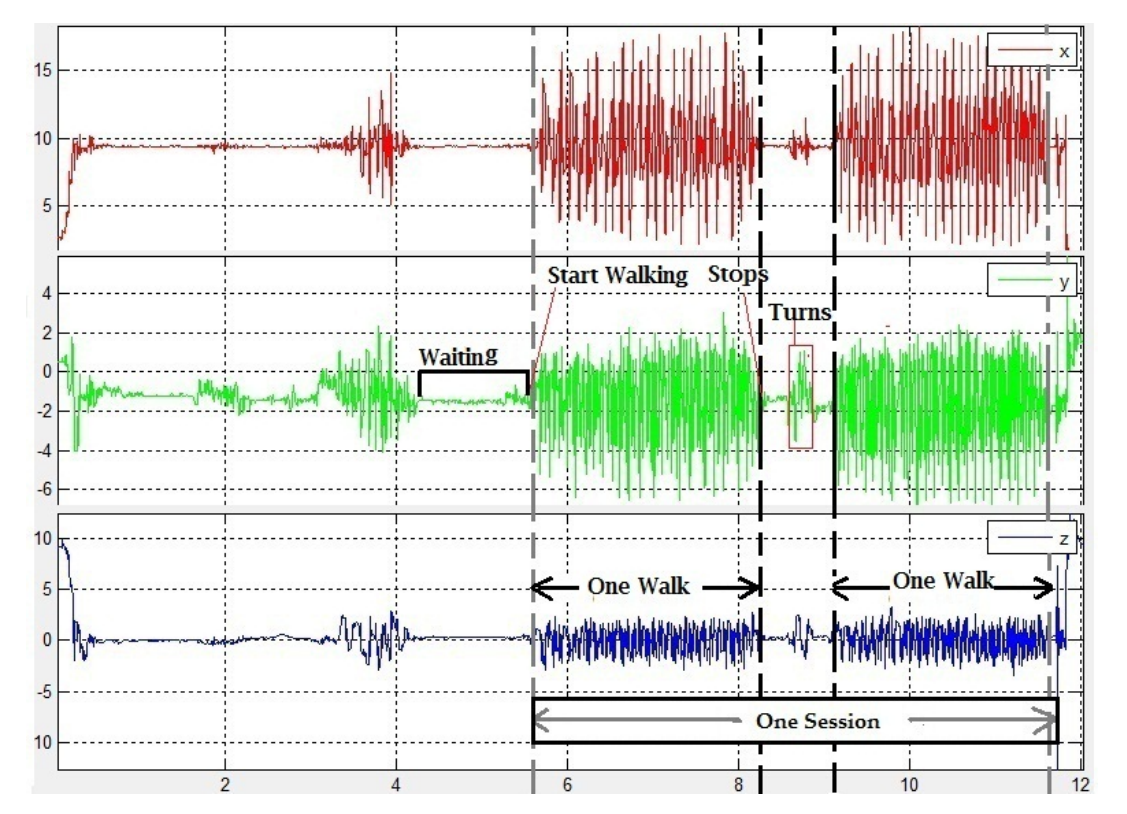
\includegraphics[width=0.8\textwidth]{Illustrations/gaitpatterns.png}
       \\
  \end{column}
  \end{columns}
\end{frame}


\subsection{}
\begin{frame}
  \frametitle{Fixed Method Approach}
  \begin{columns}
  \begin{column}{0.4\textwidth}
  \begin{itemize}
  	\item 51 Subjects
  	\linebreak
    \item Phone Clipped to Waist 
  	\linebreak
  	\item Walked Down 18.5 Meter Hallway
  	\linebreak
  	\item Separated into "Walks"
  \end{itemize}
  \end{column}
  \begin{column}{0.8\textwidth}
   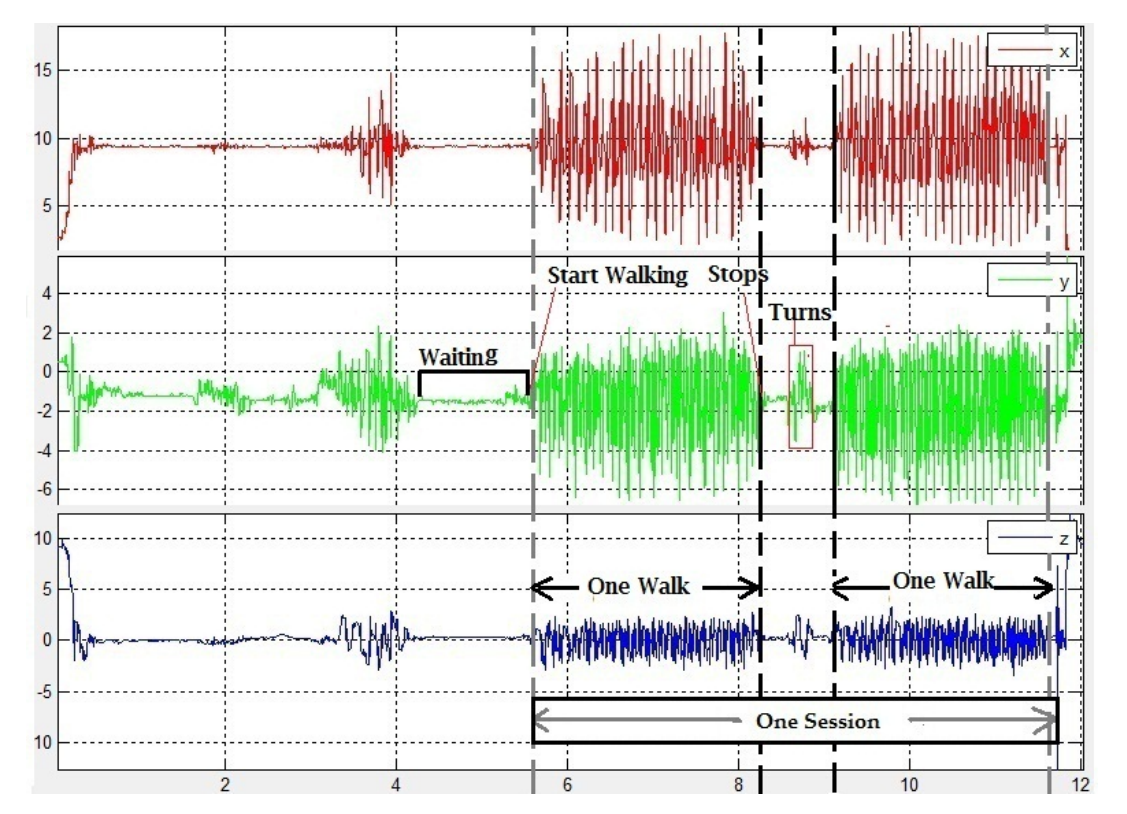
\includegraphics[width=0.8\textwidth]{Illustrations/gaitpatterns.png}
       \\
  \end{column}
  \end{columns}
\end{frame}

\subsection{}
\begin{frame}
  \frametitle{Unfixed Method Approach}

  \begin{columns}
  \begin{column}{0.6\textwidth}
  \begin{itemize}
  	\item 47 Subjects
  	\linebreak
    \item Phone in more natural location (pocket, handbag, backpack)
  	\linebreak
  	\item Performed in Real-world Environments
  	\linebreak
  	\item Separated Into Frames
  \end{itemize}
  \end{column}
  \begin{column}{0.7\textwidth}
   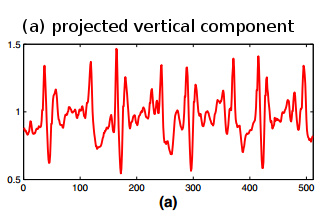
\includegraphics[width=0.6\textwidth]{Illustrations/frame.jpg}
       %http://www.smc2012.org/images/jain3-1.jpg
  \end{column}
  \end{columns}
\end{frame}





\section[Preprocessing the data]{Preprocessing The Data}

\subsection{What is Preprocessing?}
\begin{frame}
  \frametitle{Preprocessing}

  \begin{columns}
  \begin{column}{0.5\textwidth}
  \begin{itemize}
    \item Separates accelerometer data into sections
    \linebreak
    \item Drops sections with little or no movement
    \linebreak
    \item Walks VS Frames
  \end{itemize}
  \end{column}

\begin{column}{0.02\textwidth}
\end{column}

\begin{column}{0.5\textwidth}

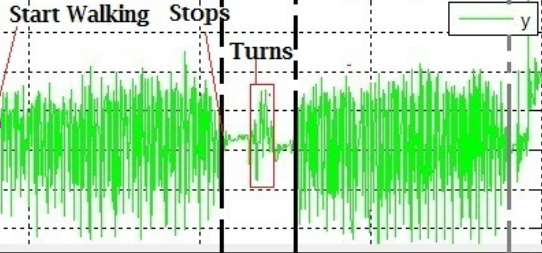
\includegraphics[width=0.91\textwidth]{Illustrations/preprocessingexample.png}

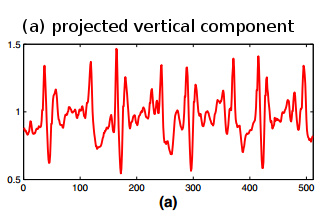
\includegraphics[width=0.91\textwidth]{Illustrations/frame.jpg}

\end{column}  
  
  
  \end{columns}
\end{frame}

\subsection{Fixed Method Preprocessing}
\begin{frame}
  \frametitle{Fixed Method Preprocessing}
  \begin{columns}
  \begin{column}{0.4\textwidth}
  \begin{itemize}
    \item Walk Extraction 
  	\linebreak
  	\item Linear Interpolation (curve fitting)
  	\linebreak
	\item Zero Normalization 
  \end{itemize}
  \end{column}  
  
\begin{column}{0.5\textwidth}

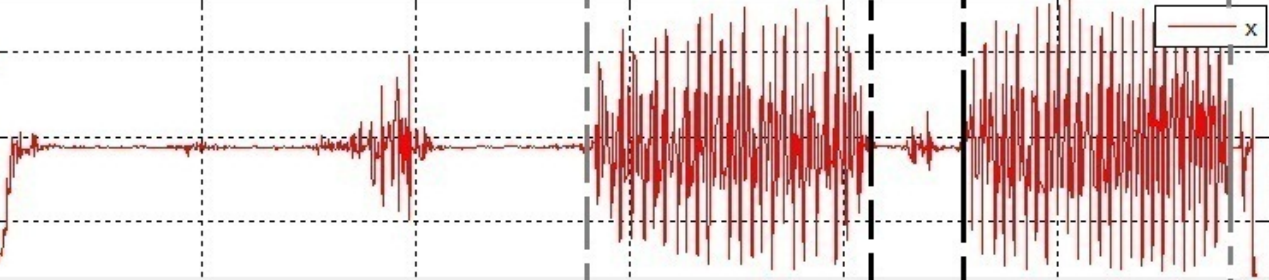
\includegraphics[width=0.91\textwidth]{Illustrations/onegaitcycle.png}

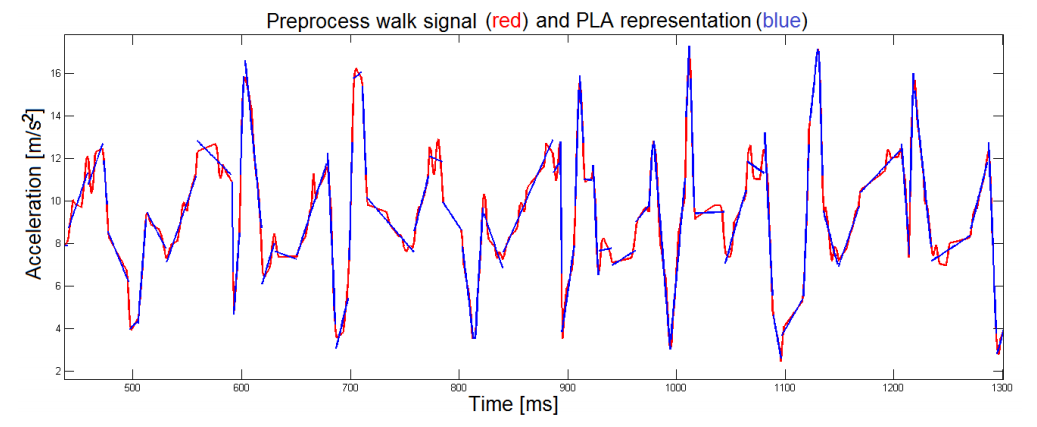
\includegraphics[width=0.91\textwidth]{Illustrations/linear.png}

\end{column}   
  
  \end{columns}
\end{frame}

\begin{frame}
  \frametitle{Walk Extraction}
  \begin{columns}
  \begin{column}{0.4\textwidth}
  \begin{itemize}
    \item Walk Extraction 
  	\linebreak
  	\item Separates walking data from non-walking data
  \end{itemize}
  \end{column}  
  
\begin{column}{0.5\textwidth}

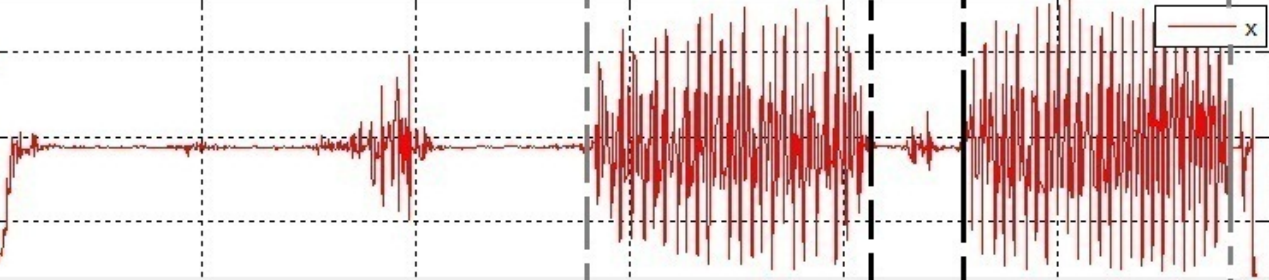
\includegraphics[width=0.91\textwidth]{Illustrations/onegaitcycle.png}

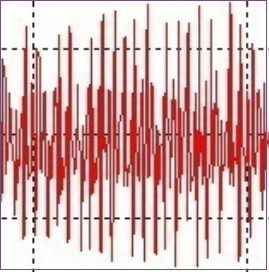
\includegraphics[width=0.51\textwidth]{Illustrations/rawgaitdata.png}

\end{column}   
  
  \end{columns}
\end{frame}

\begin{frame}
  \frametitle{Linear Interpolation}
  \begin{columns}
  \begin{column}{0.4\textwidth}
  \begin{itemize}
  	\item Linear Interpolation (curve fitting)

  \end{itemize}
  \end{column}  
  
\begin{column}{0.6\textwidth}

%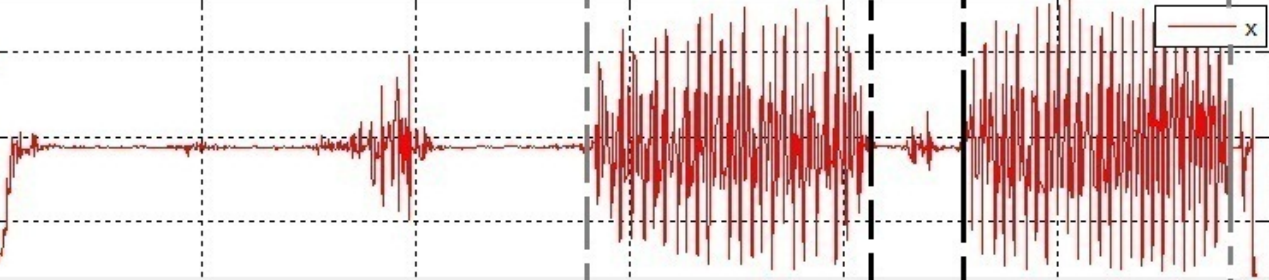
\includegraphics[width=0.91\textwidth]{Illustrations/onegaitcycle.png}

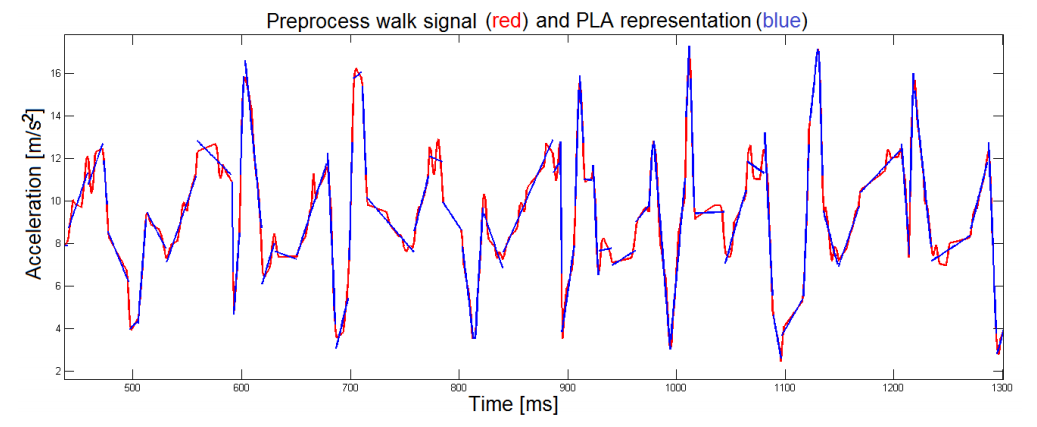
\includegraphics[width=0.91\textwidth]{Illustrations/linear.png}

\end{column}   
  
  \end{columns}
\end{frame}

\begin{frame}
  \frametitle{Zero Normalization}
  \begin{columns}
  \begin{column}{0.4\textwidth}
  \begin{itemize}
    \item Zero Normalization 
  	\linebreak
  	\item Only need the axis influenced by gravity
  	\linebreak
  	\item Acceleration along the other two axes must be zero
  \end{itemize}
  \end{column}  
  
\begin{column}{0.5\textwidth}

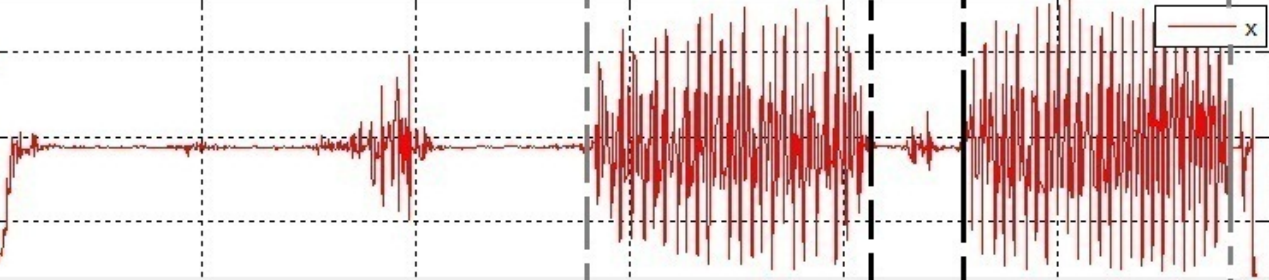
\includegraphics[width=0.95\textwidth]{Illustrations/onegaitcycle.png}

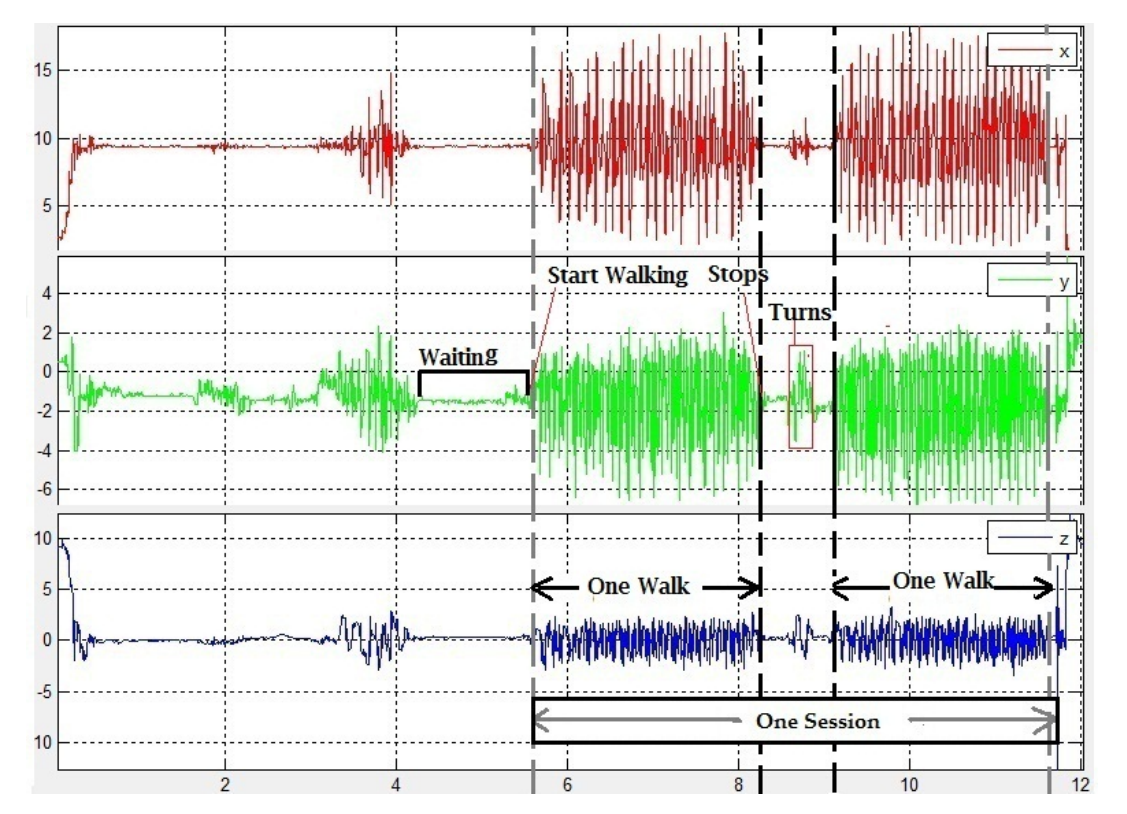
\includegraphics[width=0.95\textwidth]{Illustrations/gaitpatterns.png}

\end{column}   
  
  \end{columns}
\end{frame}

%\subsection{Unfixed Preprocessing}
%\begin{frame}
%  \frametitle{Unfixed Method Overview}
%  \begin{columns}
%  \begin{column}{1\textwidth}
%  \begin{itemize}
%  
%  	\item Three Experiments:
% 	\begin{itemize}
% 		\item Training Walking Detector
% 		\linebreak
% 		\item Evaluating Supervised Training Data
% 		\linebreak
% 		\item Unsupervised Training
% 	\end{itemize}
% 	
%  \end{itemize}
%  \end{column}
%  \begin{column}{0.7\textwidth}
%   %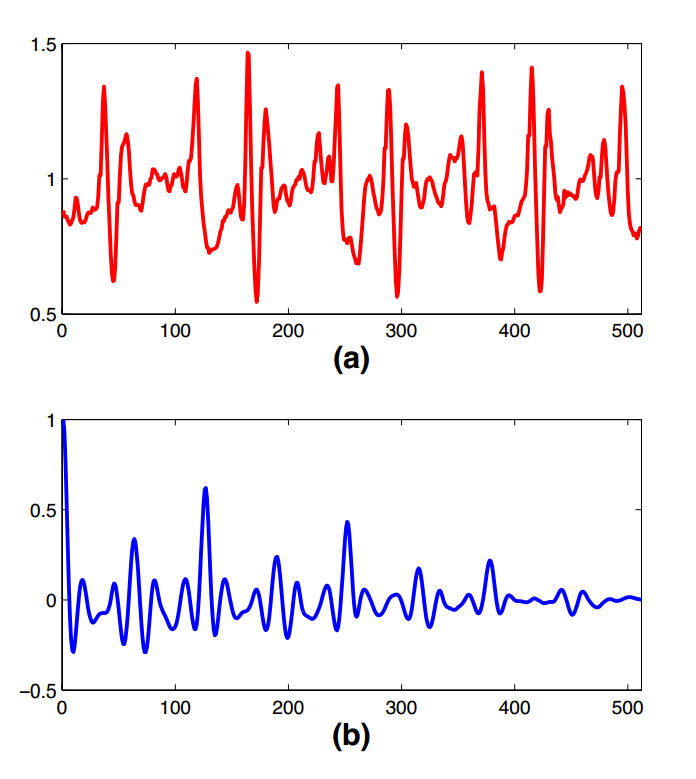
\includegraphics[width=0.7\textwidth]{Illustrations/ab.png}  
%  \end{column}
%  \end{columns}
%\end{frame}
\subsection{Unfixed Method Preprocessing}

\begin{frame}
  \frametitle{Unfixed Method Preprocessing}
  \begin{columns}
  \begin{column}{0.5\textwidth}
  	\begin{itemize}
  		\item Framing   
  		\linebreak
  		\item Projection                     
  	\end{itemize}
  \end{column}
\begin{column}{0.5\textwidth}

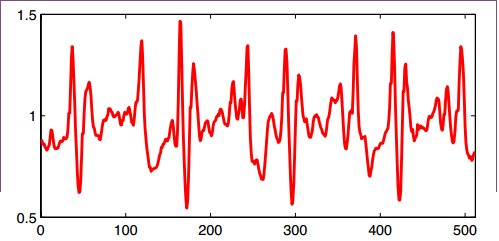
\includegraphics[width=0.95\textwidth]{Illustrations/Framing.png}

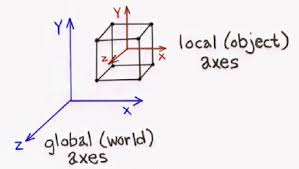
\includegraphics[width=0.95\textwidth]{Illustrations/global.jpg}
\end{column} 
  \end{columns}
\end{frame}

\begin{frame}
  \frametitle{Framing}
  \begin{columns}
  \begin{column}{0.65\textwidth}
  	\begin{itemize}
  		\item Separating Data into Equal Sections    
  		\linebreak
  		\item Frame Length: 5.12 seconds       
  		\linebreak
  		\item Each Frame contains 512 Samples
  		\linebreak
  		\item Stationary frames are dropped                
  	\end{itemize}
  \end{column}
  \begin{column}{0.6\textwidth}
   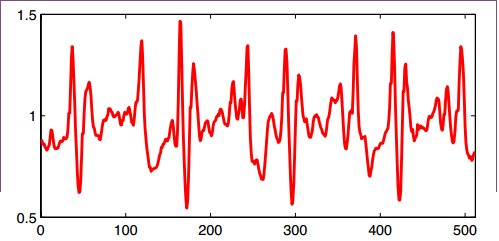
\includegraphics[width=0.8\textwidth]{Illustrations/Framing.png}
       \\
  \end{column}
  
  \end{columns}
\end{frame}

\begin{frame}
  \frametitle{Projection}
  \begin{columns}
  \begin{column}{.7\textwidth}
  
  	\begin{itemize}
  		\item Each sample is projected onto a global coordinate system (sample = {x, y, and z})
  		\linebreak
  		\item Estimating direction of gravity with changes in x, y, and z. 
  		\linebreak
%  		\item Each sample is split into two vectors: 
%  			\begin{itemize}
%  				\item Vertical (x)
%  				\item Horizontal (y, z)
%  				\linebreak
%			\end{itemize}
  		\item Frame dropped if orientation is changed  
  	\end{itemize}
  
  \end{column}
  
  \begin{column}{0.7\textwidth}
   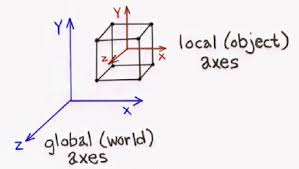
\includegraphics[width=0.5\textwidth]{Illustrations/global.jpg}
   \\
   %\only{\tiny{http://viz.aset.psu.edu/gho/sem_notes/3d_fundamentals/gifs/local_global_axes.gif}}

       
  \end{column}
  
  \end{columns}
\end{frame}




\section[Feature Extraction]{Feature Extraction}

\subsection{What is Feature Extraction?}
\begin{frame}
  \frametitle{What is Feature Extraction?}
  \begin{columns}
  \begin{column}{.9\textwidth}
  \begin{itemize}
  	\item Feature extraction separates "walking" cycles from "non-walking" cycles
  \end{itemize}
  \end{column}
  \begin{column}{0.6\textwidth}
   %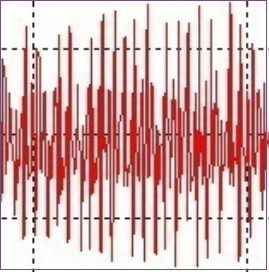
\includegraphics[width=0.6\textwidth]{Illustrations/rawgaitdata.png}
       \\
  \end{column}
  \end{columns}
\end{frame}

\subsection{Fixed Method Feature Extraction}
\begin{frame}
  \frametitle{Fixed Method Feature Extraction}
  \begin{columns}
  \begin{column}{.5\textwidth}
  \begin{itemize}
  	\item Four Steps:
  	\begin{itemize}
  		\item Cycle Length Estimation
  		\linebreak
  		\item Cycle Detection
  		\linebreak
  		\item Cycle length normalization
  		\linebreak
  		\item Omitting Unusual Cycles
  	\end{itemize}
  \end{itemize}
  \end{column}
  \begin{column}{0.6\textwidth}
   %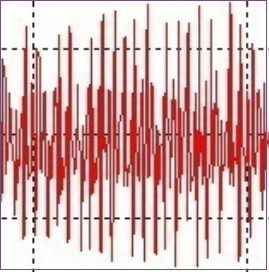
\includegraphics[width=0.6\textwidth]{Illustrations/rawgaitdata.png}
       \\
  \end{column}
  \end{columns}
\end{frame}

\begin{frame}
  \frametitle{Cycle Length Estimation}
  \begin{columns}
  \begin{column}{.5\textwidth}
  \begin{itemize}
  	\item Compute the Minimum Salience Vector of each cycle
  	\linebreak
  	\item Minimum Salience Vector
  		\begin{itemize}
  			\item Contains one entry for each data point
  			\item Each entry is the count of data values between the current value and following smaller value
  		\end{itemize}
  \end{itemize}
  \end{column}
    \begin{column}{0.7\textwidth}
   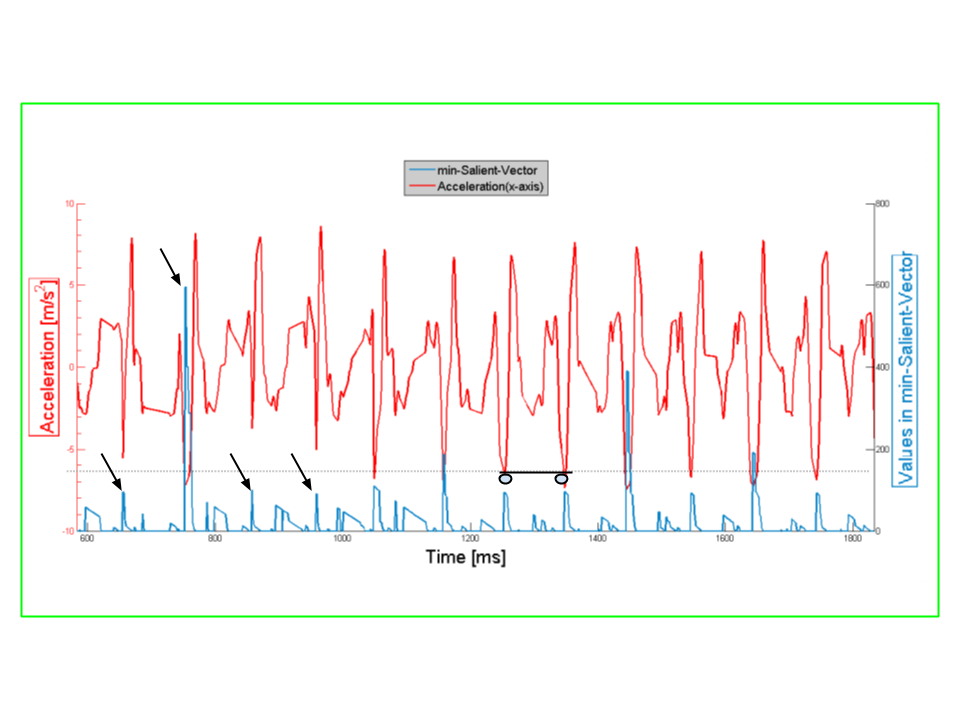
\includegraphics[width=0.8\textwidth]{Illustrations/svector2.png}
       \\
  \end{column}
  \end{columns}
\end{frame}

\begin{frame}
  \frametitle{Cycle Detection}
  \begin{columns}
  \begin{column}{.5\textwidth}
  \begin{itemize}
  	\item Detecting Individual Cycles
  	\item Start of each cycle is located using the entry with the greatest value
  	\item Spikes show the length of each cycle
  	\item Long cycles are split again using the same method
  \end{itemize}
  \end{column}
    \begin{column}{0.7\textwidth}
   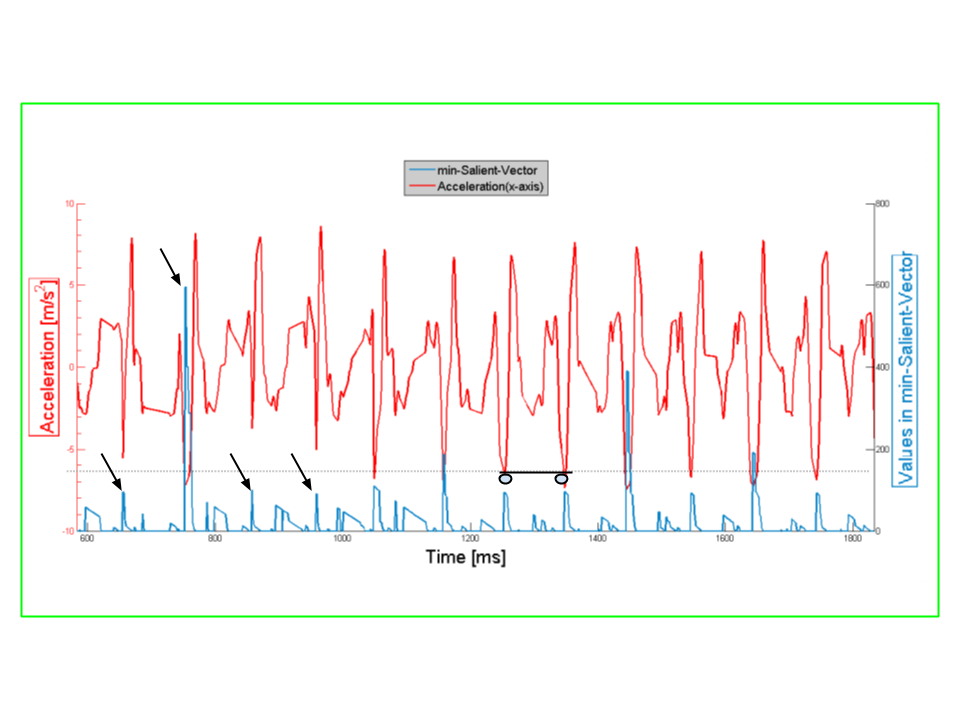
\includegraphics[width=0.8\textwidth]{Illustrations/svector2.png}
       \\
  \end{column}
  \end{columns}
\end{frame}

\begin{frame}
  \frametitle{Cycle Length Normalization}
  \begin{columns}
  \begin{column}{.55\textwidth}
  \begin{itemize}
  	\item The distance of each cycle is measured from the start of one cycle to the start of the following. 
  	\linebreak
  	\item Cycles need to be of a set length for later Gait Analysis
  	\linebreak
  	\item Linear Interpolation helps to normalize the data
  \end{itemize}
  \end{column}
    \begin{column}{0.7\textwidth}
   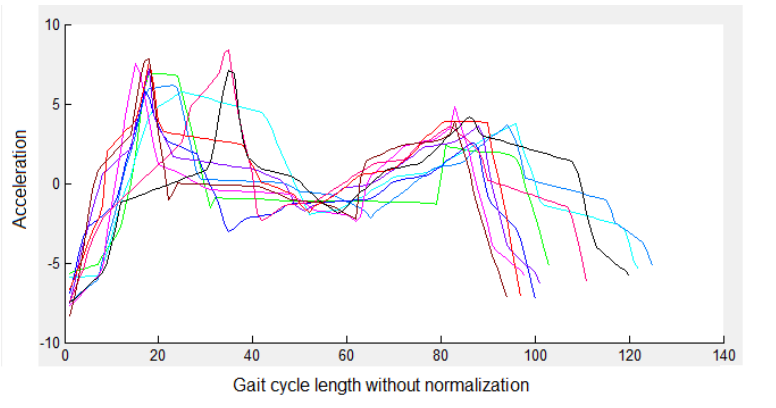
\includegraphics[width=0.7\textwidth]{Illustrations/nonnormalized.png}
       \\
  \end{column}
  \end{columns}
\end{frame}

\begin{frame}
  \frametitle{Omitting Unusual Cycles}
  \begin{columns}
  \begin{column}{.5\textwidth}
  \begin{itemize}
  	\item Deleting Unusual Gait Cycles
  	\linebreak
  	\item Dynamic Time Warping (DTW): An algorithm used to measure similarity between two sequences
  	\linebreak
  	\item Euclidean VS DTW
  	\linebreak
  	\item Cycles with half the distance of the average cycle are dropped
  \end{itemize}
  \end{column}
    \begin{column}{0.6\textwidth}
   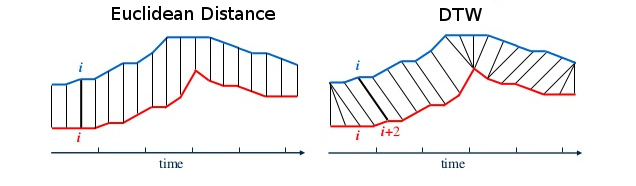
\includegraphics[width=0.9\textwidth]{Illustrations/DTW.jpg}
       
       %\only{\tiny{ http://www.slideshare.net/Henry_cu/eage2012-dtw-hvdb}}
  \end{column}
  \end{columns}
\end{frame}

%////////////////////////////////////////////////////////////////////////////////////////////////////////////
\subsection{Unfixed Feature Extraction}

\begin{frame}
  \frametitle{Unfixed Method Feature Extraction}
  \begin{columns}
  \begin{column}{.5\textwidth}
  \begin{itemize}
  	\item Three Steps:
  	\begin{itemize}
  		\item Feature Extraction I
  		\linebreak
  		\item Walking Detection
  		\linebreak
  		\item Feature Extraction II
  	\end{itemize}
  \end{itemize}
  \end{column}
  \begin{column}{0.6\textwidth}
   %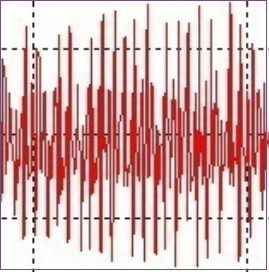
\includegraphics[width=0.6\textwidth]{Illustrations/rawgaitdata.png}
       \\
  \end{column}
  \end{columns}
\end{frame}



\begin{frame}
\frametitle{Feature Extraction I}
	\begin{itemize}
		\item Determine differences between "walking" and "non-walking"
		\linebreak
		\item Walking 1-2Hz vs Running >3Hz 
		\linebreak
		\item These features are used in Walking Detection
		
	\end{itemize}
	
\end{frame}

\begin{frame}
\frametitle{Walking Detection}
	\begin{itemize}
		\item Three classifications:
			\begin{itemize}
				\item Walking: 1-2Hz
				\linebreak
				\item Non-Walking: >3Hz (running, biking, in moving vehicle)
				\linebreak
				\item Random Movements: >0Hz (transitional movements, short spikes)
				\linebreak
			\end{itemize}
			
		\item Cycles labeled as walking move onto the next step
	\end{itemize}
\end{frame}

\begin{frame}
\frametitle{Feature Extraction II}
	\begin{itemize}
		\item Once Walking Detection confirms that the frame contains walking data, more relevant features are extracted
		\linebreak
		
		\item Some features extracted using Autocorrelation
		
		
%		\item Two sets of features extracted:
%		
%		\begin{itemize}
%			\item Fundamental Frequency of Movement
%			\item Autocorrelation Features
%		\end{itemize}



	\end{itemize}
\end{frame}

%\begin{frame}
%\frametitle{Fundamental Frequencies}
%	\begin{itemize}
%		\item This first set of features computed in this stage is the Compressed Sub-band Cepstral Coefficients (CSCC) 
%		\item CSCC based of off feature set for audio analysis.
%		\item CSCC evolves 3 steps:
%		\begin{itemize}
%			\item[1)] The energy spectrum is computed using the Fast Fourier Transform (FFT)
%			\item[2)] Then the energy spectrum is mapped into 26 bands
%			\item[3)] The discrete cosine transform of the sub-band energy is taken to form a 12-dimension vector representation
%		\end{itemize}
%	\end{itemize}
%\end{frame}

\begin{frame}
\frametitle{Autocorrelation}
 \begin{columns}
  \begin{column}{.6\textwidth}
  \begin{itemize}
		\item Useful to find periodicity and cadence of a cycle
		\linebreak
		\item Example: Phone inside a pocket
		\linebreak
		\item Segmentation methods, like minimum salience vectors, cannot be used
		\linebreak
		\item Autocorrelation can reveal features even with noise
  \end{itemize}
  \end{column}
  \begin{column}{0.65\textwidth}
   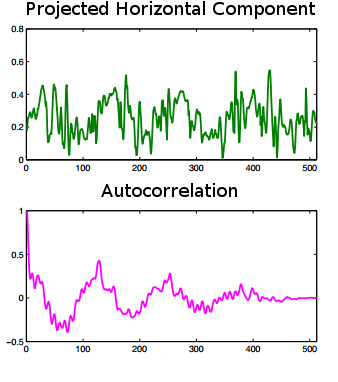
\includegraphics[width=0.6\textwidth]{Illustrations/autocorrelationcd.png}
       \\
  \end{column}
  \end{columns}  
  
\end{frame}
%/////////////////////////////////////////////////////////////////////////////////////////////////////////////////////////////////////////
\section[Gait Classification]{Gait Classification}

\subsection{Overview}
\begin{frame}
\frametitle{What is Gait Classification?}
 \begin{columns}
  \begin{column}{.9\textwidth}
  \begin{itemize}
  		\item Gait Classification determines if the user is "genuine" or an "impostor"
  \end{itemize}
  \end{column}
  \begin{column}{0.7\textwidth}
   %includegraphics[width=0.7\textwidth]{Illustrations/autocorrelation.png}
       \\
  \end{column}
  \end{columns}  
\end{frame}

\subsection{Fixed Method Gait Classification}
\begin{frame}
\frametitle{Fixed Method Gait Classification}
 \begin{columns}
  \begin{column}{.7\textwidth}
  \begin{itemize}
				\item Template-based 
				\linebreak
				\item Machine Learning 
			
  \end{itemize}
  \end{column}
  \begin{column}{0.4\textwidth}
   %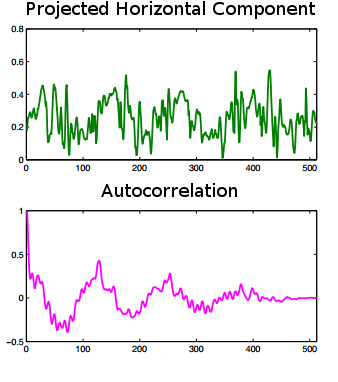
\includegraphics[width=0.6\textwidth]{Illustrations/autocorrelationcd.png}
       \\
  \end{column}
  \end{columns}  
  
\end{frame}


\begin{frame}
\frametitle{Template-based}
 \begin{columns}
  \begin{column}{.9\textwidth}
  \begin{itemize}
		\item Feature Cycle: The cycle with the lowest DTW distance 
		\linebreak
		\item Probe Cycles: The remaining cycles
		\linebreak
		\item After computing probe and reference cycles for all walks two classes are made:
			\begin{itemize}
			\item Genuine
			\item Impostor
			\linebreak
			\end{itemize}
		
		\item Genuine and Impostor are made by comparing the DTW distance of all the reference and probe cycles					
		\linebreak
		\item 50\% of the Probe cycles must be classified as genuine		
  \end{itemize}
  \end{column}
  \begin{column}{0.7\textwidth}
   %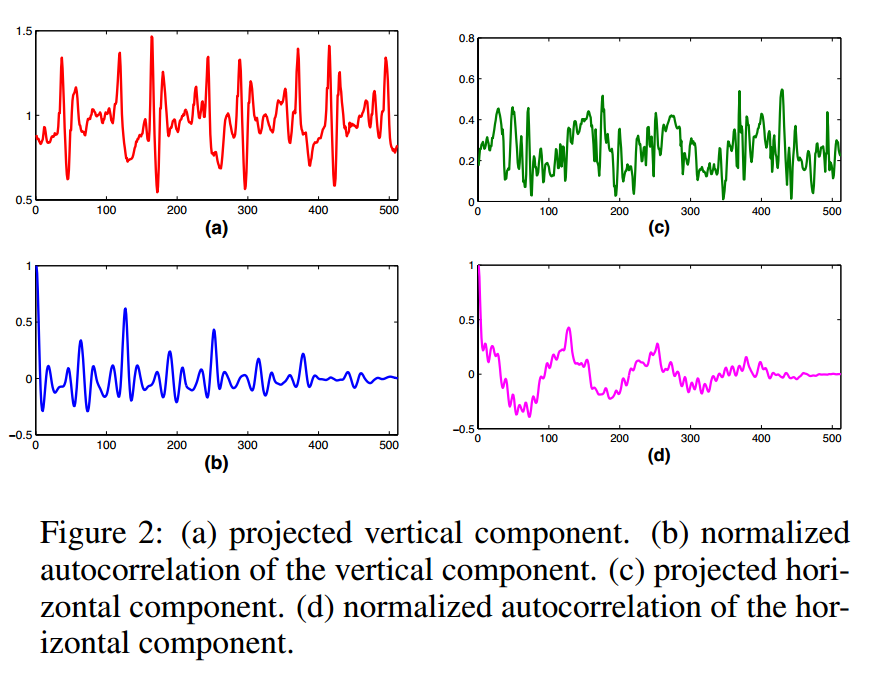
\includegraphics[width=0.7\textwidth]{Illustrations/autocorrelation.png}
       \\
  \end{column}
  \end{columns}  
\end{frame}

\begin{frame}
\frametitle{Machine Learning}
 \begin{columns}
  \begin{column}{.65\textwidth}
  \begin{itemize}
  		\item Data is split into two groups:
  			\begin{itemize}
  				\item Training (80\%)
  				\item Testing (20\%)
  				\linebreak
  			\end{itemize}
		\item Support Vector Machines (SVMs) are used for biometric classification
		\linebreak
		\item A SVM finds a hyperplane that linearly separates data into two classes: genuine and impostor
  \end{itemize}
  \end{column}
  \begin{column}{0.6\textwidth}
   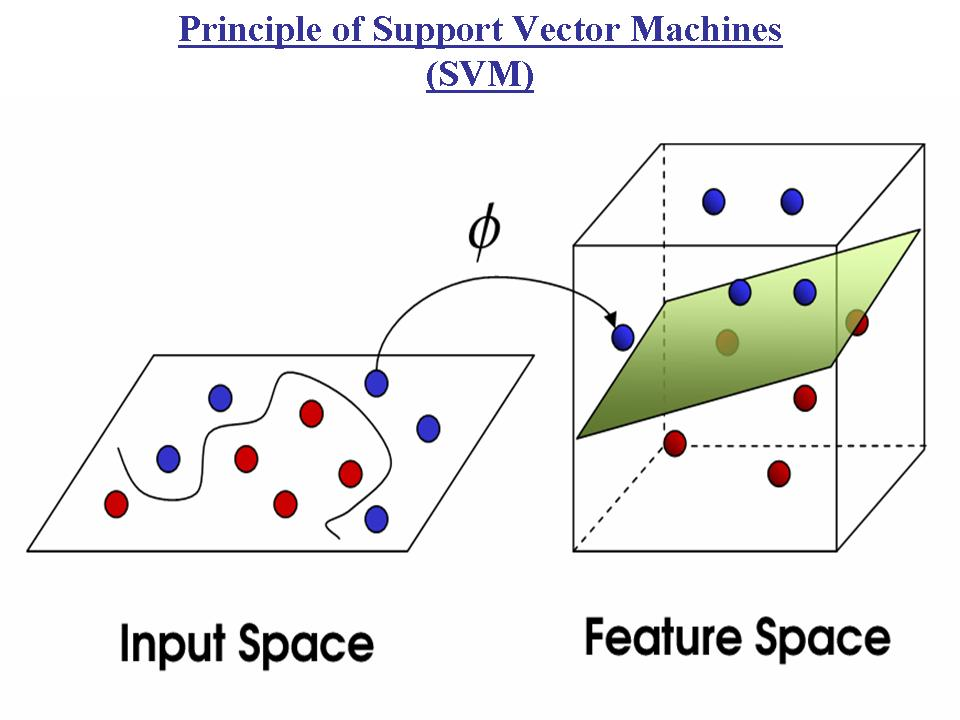
\includegraphics[width=0.6\textwidth]{Illustrations/svm.jpg}
       \\
  \end{column}
  \end{columns}  
\end{frame}

\begin{frame}
\frametitle{Machine Learning}
 \begin{columns}
  \begin{column}{.6\textwidth}
  \begin{itemize}
  		\item The data is not usually linearly separable. Therefore, a kernel function is used.
		\item A kernel function maps non linearly separable data to a high dimension space 
		\item These data points are now compared to the Testing data set and labelled as genuine or imposter
		\item Classification: Class with the most data points
  \end{itemize}
  \end{column}
  \begin{column}{0.6\textwidth}
   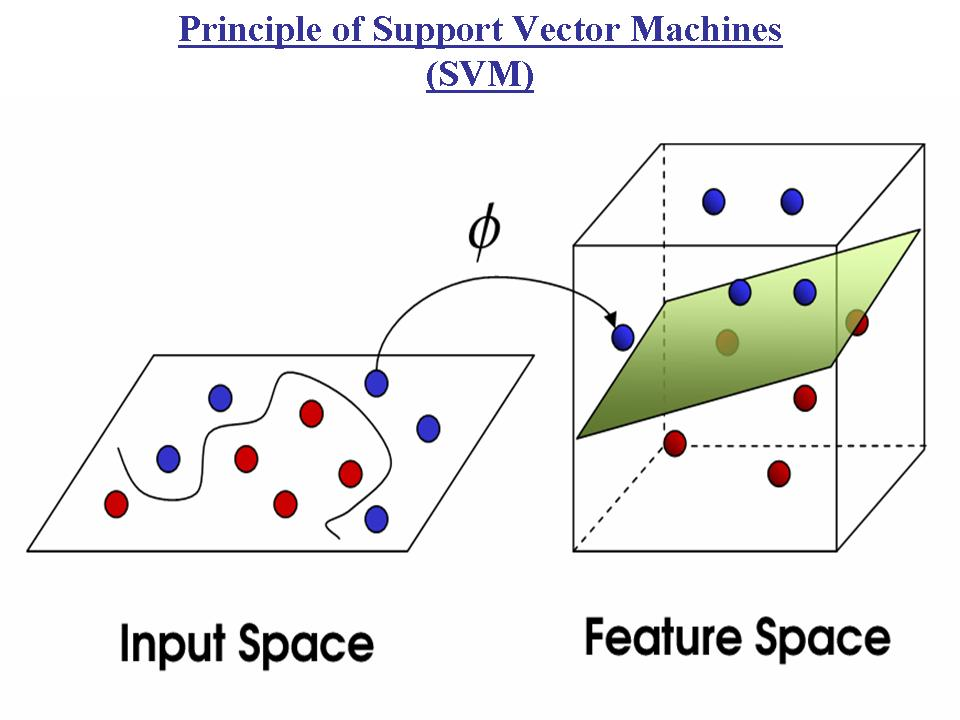
\includegraphics[width=0.6\textwidth]{Illustrations/svm.jpg}
       \\
  \end{column}
  \end{columns}  
\end{frame}

\subsection{Unfixed Method Gait Classification}
\begin{frame}
\frametitle{Unixed Method Gait Classification}
 \begin{columns}
  \begin{column}{.9\textwidth}
			\begin{itemize}
				\item Universal Background Model: 
				\begin{itemize}
					\item Data Pooled from a group of subjects
					\item Represents various gait patterns
				\end{itemize}	
			\end{itemize}
  \end{column}
  \begin{column}{0.4\textwidth}
   %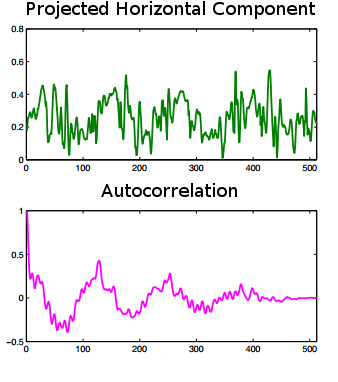
\includegraphics[width=0.6\textwidth]{Illustrations/autocorrelationcd.png}
       \\
  \end{column}
  \end{columns}  
  
\end{frame}
 \begin{frame}
\frametitle{Unfixed Method }
 \begin{columns}
  \begin{column}{.9\textwidth}
  \begin{itemize}
		\item The UBM is trained with a user's data
		\linebreak
		\item The current user's gait model is generated from the extracted features
		\linebreak
		\item The current user's model is compared to the personalized Universal Background Model and either accepts or rejects.
		\linebreak
		\item Further training of the UBM is done by recording false negatives
  \end{itemize}
  \end{column}
  \begin{column}{0.2\textwidth}
   %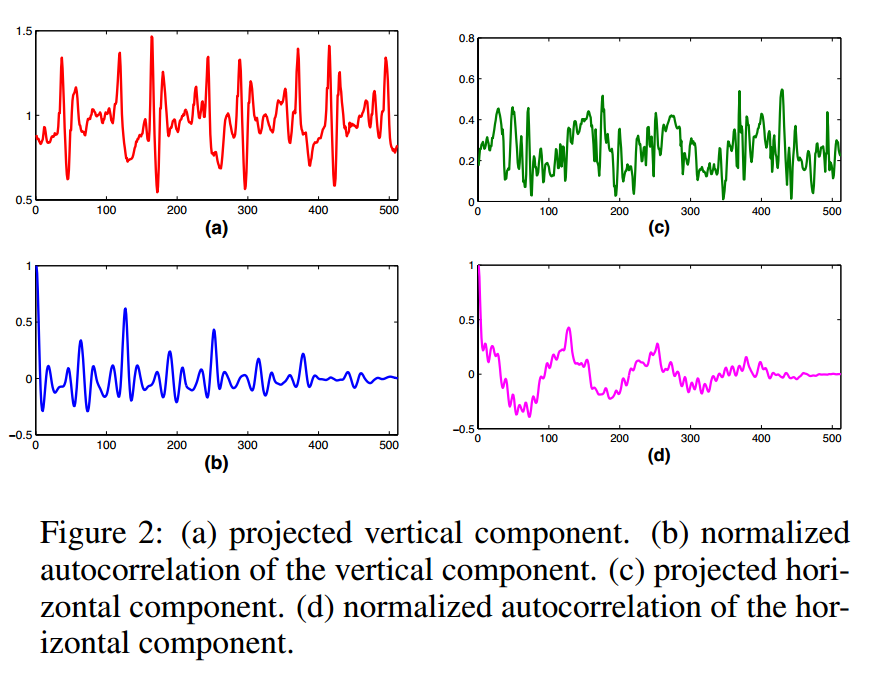
\includegraphics[width=0.7\textwidth]{Illustrations/autocorrelation.png}
       \\
  \end{column}
  \end{columns}  
\end{frame}

\section[Results]{Results}
\begin{frame}
\frametitle{Conclusions}
	\begin{itemize}
		\item Accuracy calculated by Equal Error Rate (EER): 
			\begin{itemize}
			\item False acceptance rate and false rejection rate are equal. 
			\item The Lower the EER the more accurate the method
			\end{itemize}
			\item EER:
			\begin{itemize}
			\item Fixed: EER 22.49\%
			\item Unfixed: EER 14\%
			\end{itemize}
			\item RunTime: 
			\begin{itemize}
				\item Fixed: 2-3 minutes
				\item Unfixed: 30 milliseconds
			\end{itemize}
				
	\end{itemize}
	
\end{frame}


\section[Conclusion]{Conclusion}
\begin{frame}
\frametitle{Conclusions}
	\begin{itemize}
		\item The unfixed method:
			\begin{itemize}
				\item Uses a real-world approach 
				\item More accurate
				\item Faster
			\end{itemize}
	\end{itemize}
	
\end{frame}






\section*{References}

\begin{frame} 
	\frametitle{References} 
	
	\begin{center}
		{\LARGE Questions?}
	\end{center}
	
\begin{itemize}
\item[1)]H.~Lu, J.~Huang, T.~Saha, and L.~Nachman, Unobtrusive gait verification for mobile phones, 2014

\item[2)] M.~Muaaz and R.~Mayrhofer, An analysis of different approaches to gait recognition using cellphone based accelerometers, 2013

\end{itemize}
%	\begin{thebibliography}{lskdjf}
%	
%	\bibitem{McPhee:2009:gecco}
%N.~F. McPhee, E.~Crane, S.~Lahr, and R.~Poli.
%\newblock Developmental Plasticity in Linear Genetic Programming.
%\newblock In G\"unther Raidl, \emph{et al}, editors, {\em GECCO '09}, pages 1019--1026, Montr\'eal, Qu\'ebec, Canada, 2009.
%	
%	\bibitem{citeulike:3452411}
%	R.~Poli and N.~McPhee.
%\newblock A linear estimation-of-distribution {GP} system.
%\newblock In M.~O'Neill, \emph{et al}, editors, {\em EuroGP 2008}, volume
%  4971 of {\em LNCS}, pages 206--217, Naples,
%  26-28 Mar. 2008. Springer.
%  
%  	\end{thebibliography}
%	
%	\linespace
%	\begin{center}
%	See the GECCO '09 paper for additional references.
%	\end{center}
\end{frame} 

\end{document}


